\documentclass{article}
\usepackage{tikz}
\usepackage{amsmath}
\usetikzlibrary{decorations.pathmorphing, arrows.meta, positioning}

\begin{document}

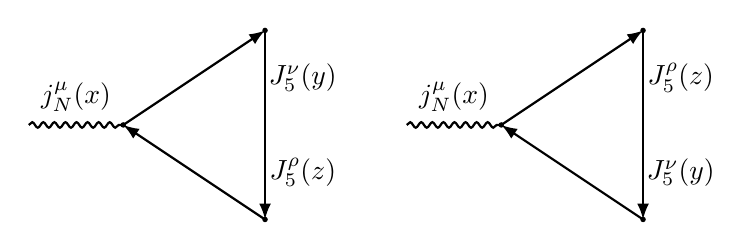
\begin{tikzpicture}[
    scale=1.2,
    thick,
    fermion/.style={-{Latex[length=2mm]}, thick},
    gluon/.style={decorate, decoration={snake, amplitude=1pt, segment length=4pt}, thick},
    vertex/.style={inner sep=0pt, minimum size=2pt, fill=black, circle}
]

% First triangle diagram (left)
\coordinate (A1) at (0,0);
\coordinate (B1) at (1.5,1);
\coordinate (C1) at (1.5,-1);

% Fermion lines for first triangle
\draw[fermion] (A1) -- (B1);
\draw[fermion] (B1) -- (C1);
\draw[fermion] (C1) -- (A1);

% Vertices for first triangle
\node[vertex] at (A1) {};
\node[vertex] at (B1) {};
\node[vertex] at (C1) {};

% Wavy line (gluon) for first triangle
\draw[gluon] (-1,0) -- (A1);

% Labels for first triangle
\node at (-0.5,0.3) {$j_N^\mu(x)$};
\node at (1.9,0.5) {$J_5^{\nu}(y)$};
\node at (1.9,-0.5) {$J_5^{\rho}(z)$};

% Second triangle diagram (right)
\coordinate (A2) at (4,0);
\coordinate (B2) at (5.5,1);
\coordinate (C2) at (5.5,-1);

% Fermion lines for second triangle
\draw[fermion] (A2) -- (B2);
\draw[fermion] (B2) -- (C2);
\draw[fermion] (C2) -- (A2);

% Vertices for second triangle
\node[vertex] at (A2) {};
\node[vertex] at (B2) {};
\node[vertex] at (C2) {};

% Wavy line (gluon) for second triangle
\draw[gluon] (3,0) -- (A2);

% Labels for second triangle
\node at (3.5,0.3) {$j_N^\mu(x)$};
\node at (5.9,0.5) {$J_5^{\rho}(z)$};
\node at (5.9,-0.5) {$J_5^{\nu}(y)$};

\end{tikzpicture}

\end{document}